% !TEX TS-program = pdflatex
% !TEX encoding = UTF-8 Unicode

% This is a simple template for a LaTeX document using the "article" class.
% See "book", "report", "letter" for other types of document.

\documentclass[11pt]{article} % use larger type; default would be 10pt

\usepackage[utf8]{inputenc} % set input encoding (not needed with XeLaTeX)
\usepackage{graphicx}
\usepackage{algorithm}
\usepackage{algorithmicx}
\usepackage{algpseudocode}
\usepackage{multirow}

%%% Examples of Article customizations
% These packages are optional, depending whether you want the features they provide.
% See the LaTeX Companion or other references for full information.

%%% PAGE DIMENSIONS
\usepackage{geometry} % to change the page dimensions
\geometry{a4paper} % or letterpaper (US) or a5paper or....
% \geometry{margin=2in} % for example, change the margins to 2 inches all round
% \geometry{landscape} % set up the page for landscape
%   read geometry.pdf for detailed page layout information

\usepackage{graphicx} % support the \includegraphics command and options

% \usepackage[parfill]{parskip} % Activate to begin paragraphs with an empty line rather than an indent

%%% PACKAGES
\usepackage{booktabs} % for much better looking tables
\usepackage{array} % for better arrays (eg matrices) in maths
\usepackage{paralist} % very flexible & customisable lists (eg. enumerate/itemize, etc.)
\usepackage{verbatim} % adds environment for commenting out blocks of text & for better verbatim
\usepackage{subfig} % make it possible to include more than one captioned figure/table in a single float
% These packages are all incorporated in the memoir class to one degree or another...

%%% HEADERS & FOOTERS
\usepackage{fancyhdr} % This should be set AFTER setting up the page geometry
\pagestyle{fancy} % options: empty , plain , fancy
\renewcommand{\headrulewidth}{0pt} % customise the layout...
\lhead{}\chead{}\rhead{}
\lfoot{}\cfoot{\thepage}\rfoot{}

%%% SECTION TITLE APPEARANCE
\usepackage{sectsty}
\allsectionsfont{\sffamily\mdseries\upshape} % (See the fntguide.pdf for font help)
% (This matches ConTeXt defaults)

%%% ToC (table of contents) APPEARANCE
\usepackage[nottoc,notlof,notlot]{tocbibind} % Put the bibliography in the ToC
\usepackage[titles,subfigure]{tocloft} % Alter the style of the Table of Contents
\renewcommand{\cftsecfont}{\rmfamily\mdseries\upshape}
\renewcommand{\cftsecpagefont}{\rmfamily\mdseries\upshape} % No bold!

%%% END Article customizations

%%% The "real" document content comes below...

\title{Lab 4: Dimensionality Reduction}
\author{Ruofan Zhou}
%\date{} % Activate to display a given date or no date (if empty),
         % otherwise the current date is printed 

\begin{document}
\maketitle

\section{Faces}
\subsection{Dimensionality of the Dataset}
1. There are \emph{5000} faces and \emph{50} measurements.\\
2.  See the \emph{variance-dimension} plot as below:\\
\centerline{
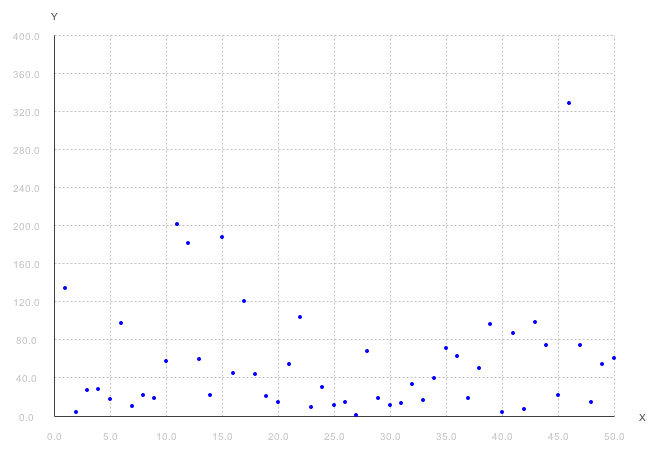
\includegraphics[width=13cm]{pic/p1}}\\
3. I perfer to describe the face with \emph{7} variable parts: \emph{hat color, hair length, hair color, eye size, face color, mouth shape, eye color}. \\
4. I sorted the variances and get the plot: \\
\centerline{
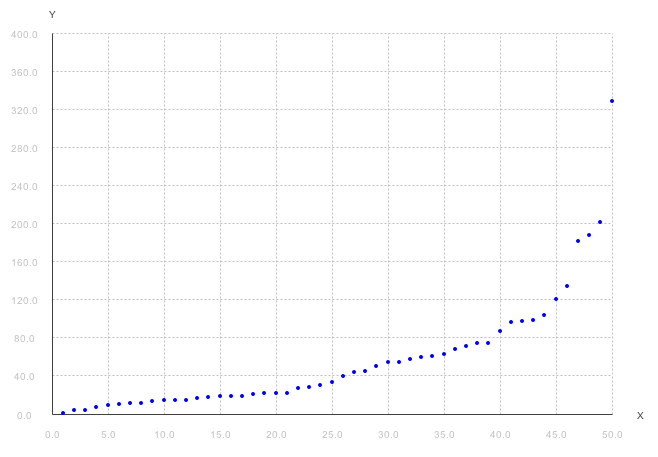
\includegraphics[width=13cm]{pic/p2}}\\
5.  \\
\subsection{Principal Component Analysis}
See file \emph{CoActorPrediction.java} to view my implementation of the classes.
\\
And I computer \emph{MyOwnScorning} with:
\\
\centerline{$\frac{N(u, v)^{2} \times \sqrt{|N(u)-N(v)|}}{N(u) + N(v)}$}
\\
In which N(i) stands for neibour number of i, and N(i, j) stands for common neibour number of i and j.
\\
And Here's accuracy of the 3 link prediction strategies: 

\begin{table}[!hbp]
\centering
\begin{tabular}{|c|c|c|}
\hline
Name & Accuracy & Improvement \\
\hline
PreferentialAttachment & 2.096\% & 3.19x \\
\hline
CommonNeighbors & 5.114\% & 7.79x \\
\hline
MyOwnScoring & 5.388\% & 8.21x \\
\hline
\end{tabular}
\end{table}

\section{Random Walks}
1. Setting N = 10000 and node u as initial seed, the average of a Facebook user is \emph{48.6725}, which still has a difference with the reference answer. The problem I think, is the \emph{algorithm itself}, and \emph{maybe node u is in a small component of the network}, and maybe \emph{the dataset itself changes}.
\\
2. I changed walk strategy in my algorithm: every time I walk across 3 people instead of one(i.e. I walk to the node's neighbor's neighbor's neighbor instead of its neighbor), and there's also a repeat judgment in my code. After changing, the estimated age becomes \emph{50.675}, which is more close to the reference answer.
\\
\subsection{Bizarre Social Networks}
1. Setting N = 10000 and using different beginning node, we get average age as below: \\

\begin{table}[!hbp]
\centering
\begin{tabular}{|c|c|c|}
\hline
Beginning Node & Average Age & Age of Beginning Node \\
\hline
u & 50.1445 & 13\\
\hline
v & 55.5635 & 39 \\
\hline
w & 64.1295 & 89 \\
\hline
\end{tabular}
\end{table}

we can see much difference between each other. And we can also find that with younger beginning node we get smaller average age and with older beginning node we get larger average age. Maybe it's the \emph{Herding} property. The friends are seems so familiar.\\
\\
2. The same strategy as above, now get the answers:\\

\begin{table}[!hbp]
\centering
\begin{tabular}{|c|c|c|}
\hline
Beginning Node & Average Age & Age of Beginning Node \\
\hline
u & 58.721 & 13\\
\hline
v & 58.2856 & 39 \\
\hline
w & 57.4979 & 89 \\
\hline
\end{tabular}
\end{table}

The answeres now become more similar :) \\


Finally, I use my strategy(this time, walk across 6 people every time) on the \emph{Directions}, get answers:\\

\begin{table}[!hbp]
\centering
\begin{tabular}{|c|c|c|}
\hline
Beginning Node & Average Age & Age of Beginning Node \\
\hline
u & 49.5636 & 23\\
\hline
v & 49.4373 & 22 \\
\hline
w & 49.4054 & 39 \\
\hline
\end{tabular}
\end{table}

So, my estimate of the average age of Directions's users is \emph{49.5}.
\end{document}
